\chapter{Аналитическая часть}

В данном разделе предоставим описание трехмерной модели объектов в сцене, рассмотрим формализацию сценариев и критерии, которым должна соответствовать программа. 
Также исследуем методы создания трехмерных изображений и моделирования освещения.

\section{Описание модели трёхмерного объекта в сцене}

В данной работе трехмерный объект в сцене описывается с использованием полигональной сетки.

Полигональная сетка -- это совокупность вершин, рёбер и граней, которые определяют форму многогранного объекта в трёхмерной компьютерной графике и объёмном моделировании~\cite{rodgers} . 
Гранями обычно являются треугольники, четырёхугольники или другие простые выпуклые многоугольники (полигоны).

Этот метод является универсальным, так как позволяет описывать трехмерные объекты в различных формах. 
Однако количество полигонов существенно влияет  на реалистичность визуализации модели, но при этом обработка большого числа граней требует больших вычислительных ресурсов.

\section{Формализация объектов синтезируемой сцены}

Сцена состоит из:

\begin{enumerate}[label={\arabic*)}]
	\item источников света -- в сфере создания трехмерных изображений
	представляют собой материальные точки, из которых исходят лучи света
	во все стороны. В некоторых случаях источник света может быть
	расположен в бесконечности и иметь определенную направленность;
	\item объектов -- в сфере создания трехмерных изображений представляют
	собой геометрической фигуры, которые касаются между собой, из
	которых строится модель;
	\item камера -- характеризуется своим пространственным положением и
	направлением просмотра.
\end{enumerate}

\section{Анализ алгоритмов построения трёхмерного изображения}

Для выбора подходящего алгоритма построения изображения, необходимо
провести обзор известных алгоритмов и осуществить выбор наиболее
подходящего для реализации поставленной задачи.

\subsection{Алгоритм, использующий Z - буфер}

Алгоритм Z - буфера –- один из простейших алгоритмов, который работает в пространстве изображения~\cite{rodgers}.

Буфер кадра выполняет функцию заполнения пикселей в изображении атрибутами интенсивности. 
Для этой задачи требуется буфер регенерации, в котором сохраняются яркостные значения, а также Z - буфер (буфер глубины), который хранит информацию о координатах z для каждого пикселя. 
В начале процесса Z - буфер заполняется минимальными значениями Z, а буфер регенерации заполняется фоновыми значениями. 
Затем многоугольники преобразуются в растровую форму и записываются в буфер регенерации. 
Важно отметить, что многоугольники не сортируются в начале процесса.

В ходе выполнения каждый новый пиксель сравнивается с пикселем в Z - буфере, и если новый пиксель находится ближе к наблюдателю, чем тот, который уже есть в буфере кадра, то новый пиксель перезаписывает существующий в буфере. 
Значение Z - буфера также корректируется, чтобы учитывать глубину нового пикселя. 
Если новый пиксель имеет меньшее значение Z, чем пиксель в буфере, то никакие действия не выполняются.

На рисунке~\ref{fig:z_buffer} представлена иллюстрация работы алгоритма Z - буфера~\cite{z_buffer}.
\begin{figure}[h]
	\begin{center}
		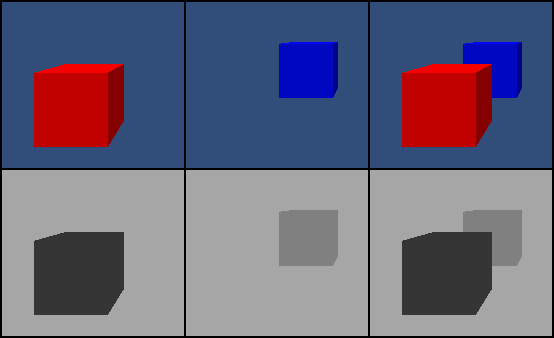
\includegraphics[width=\linewidth]{photos/z_buffer2.png}
	\end{center}
	\caption{Иллюстрация работы алгоритма Z - буфера}
	\label{fig:z_buffer}
\end{figure}

Преимущества этого алгоритма:
\begin{itemize}
	\item Простота. Сцены могут быть любой сложности.
	\item Элементы сцены не нужно сортировать.
\end{itemize}

Недостатки:
\begin{itemize}
	\item Большой объём памяти.
	\item Трудоёмкость устранения лестничного эффекта.
	\item Трудоёмкость реализации эффектов прозрачности и просвечивания.
\end{itemize}

\subsection{Алгоритм обратной трассировки лучей}

Алгоритм предлагает следующий подход: для каждого пикселя на изображении мы проводим луч, начинающийся от камеры, и программа должна определить, где этот луч пересекается со сценой. 
Этот исходный луч называется первичным лучом~\cite{lectures}.

На рисунке~\ref{fig:ray_trace} показан пример, когда первичный луч пересекает объект и достигает точки H1:
\begin{figure}[h]
	\begin{center}
		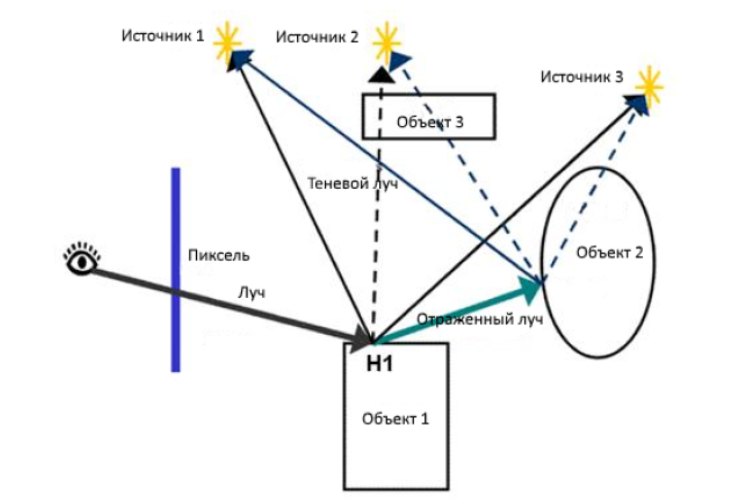
\includegraphics[width=\linewidth]{photos/tras.png}
	\end{center}
	\caption{Иллюстрация работы алгоритма обратной трассировки лучей}
	\label{fig:ray_trace}
\end{figure}

Алгоритм начинает с проверки видимости точки для источника света. 
Для этого он выпускает теневой луч из этой точки к источнику света. 
Если луч пересекает какой-либо объект сцены, это означает, что точка находится в тени и не нуждается в освещении. 
В противном случае, программа определяет степень освещенности точки.

Затем алгоритм анализирует отражающие и преломляющие свойства объекта. Если такие свойства присутствуют, из точки H1 испускается отраженный луч, и процесс повторяется рекурсивно. 
То же самое происходит при рассмотрении явления преломления. 
Этот алгоритм эффективно решает поставленную задачу и обеспечивает высокую степень реалистичности полученного изображения. 
Кроме того, он учитывает все физические явления, такие как отражение, преломление и создание теней~\cite{lectures}.

Преимущества этого алгоритма:
\begin{itemize}
	\item Высокая степень реализма. Метод обратной трассировки лучей позволяет создавать изображения с высокой степенью детализации и реализма, включая отражения, преломления, тени и другие эффекты.
	\item Гибкость. Метод обратной трассировки лучей позволяет создавать различные типы изображений, включая статические и анимированные, а также работать с различными типами материалов и источников света.
	\item Возможность использования параллельных вычислений. Метод обратной трассировки лучей может быть эффективно распараллелен на множество процессоров или ядер, что позволяет ускорить процесс создания изображения.
\end{itemize}

Недостатки:
\begin{itemize}
	\item Высокая вычислительная сложность. Метод обратной трассировки лучей требует большого количества вычислительных ресурсов, что может привести к длительным временам обработки и высоким затратам на оборудование.
	\item Проблемы с прозрачностью. Метод обратной трассировки лучей может столкнуться с проблемами при работе с прозрачными объектами, такими как стекло или вода, которые могут создавать шум и артефакты на изображении.
\end{itemize}

\subsection*{Вывод}

Был выбран алгоритм обратной трассировки лучей с целью исключения невидимых линий и поверхностей. 
Этот подход обеспечивает создание изображений с высокой степенью реалистичности, учитывая различные физические и оптические явления, и также предоставляет возможность взаимодействия с телами, поддерживающими вращение.

\section{Анализ алгоритмов моделирования освещения}

Реалистичность изображения сильно зависит от правильного выбора алгоритма освещения. 
Существует две основные группы моделей освещенности: локальные и глобальные. 
Локальные модели уделяют внимание только первичным источникам света, в то время как глобальные модели также учитывают физические явления, такие как отражение света от поверхностей и преломление света.

Для выбора подходящего алгоритма  моделирования освещения, необходимо
провести обзор известных алгоритмов и осуществить выбор наиболее
подходящего для реализации поставленной задачи.

\subsection{Модель Ламберта}

В этой модели рассматривается идеальное диффузное освещение, где свет, попавший на поверхность, рассеивается равномерно во всех направлениях. 
При расчетах учитываются только ориентация поверхности (представленная нормалью $\overline{N}$)  и направление света (представленное вектором $\overline{L}$). 
Обозначим $I_d$ как рассеянную составляющую освещенности в конкретной точке, $K_d$ как свойство материала отражать рассеянное освещение, и $I_0$ как интенсивность рассеянного освещения.

С учетом этих параметров, интенсивность освещения можно рассчитать по следующей формуле:
\begin{equation}
	I_d = K_d(\overline{L}, \overline{N})I_0.
	\label{fig:equation_1}
\end{equation}

Модель Ламберта является одной из наиболее простых моделей освещения, и она часто используется в сочетании с другими моделями, так как диффузная составляющая присутствует в большинстве сценариев~\cite{lambert}.

\subsection{Модель Фонга}

Модель Фонга разделяет освещенность в каждой точке на три компоненты~\cite{lambert}:
\begin{itemize}
	\item Фоновое освещение: Это светлое фоновое освещение, которое всегда присутствует и не зависит от источников света. Оно считается постоянным для всей сцены.
	\item Рассеянный свет: Это освещение, которое зависит от угла, под которым свет падает на поверхность, и угла между нормалью поверхности и вектором, указывающим на источник света. Это отвечает за равномерное освещение поверхности.
	\item Бликовая составляющая: Это освещение, которое отражает свет от бликовых точек на поверхности. Оно зависит от того, насколько близки вектор отраженного света к вектору, указывающему на наблюдателя.
\end{itemize}

Свойства источников света определяют мощность каждой из этих компонент, а свойства материала объекта определяют, как материал взаимодействует со светом.

Пусть: 

\begin{itemize}
	\item $\overline{N}$ – вектор нормали к поверхности в точке;	
	\item $\overline{L}$ – падающий луч;
	\item $\overline{R}$ – отражённый луч; 
	\item $\overline{V}$ – вектор, направленный к наблюдателю; 
	\item $k_a$ – коэффициент фонового освещения;
	\item $k_d$ – коэффициент диффузного освещения;
	\item $k_s$ – коэффициент зеркального освещения; 
	\item p – степень, аппроксимирующая пространственное распределение зеркально отражённого света.  	
\end{itemize}
Тогда интенсивность света вычисляется с использованием формулы~\ref{fig:equation_2}:
\begin{equation}
	I_a = K_a * I_a + K_d(\overline{N}, \overline{L}) +  K_s(\overline{R}, \overline{V})^p.
	\label{fig:equation_2}
\end{equation}
На рисунке~\ref{fig:fongo1} показан пример работы модели Фонга:
\begin{figure}[h]
	\begin{center}
		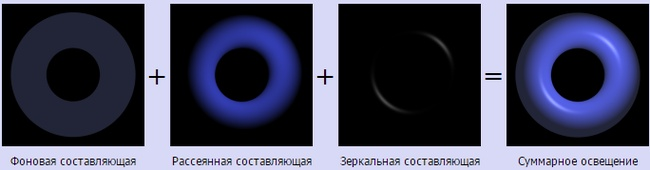
\includegraphics[width=\linewidth]{photos/fonga.png}
	\end{center}
	\caption{Иллюстрация работы модели Фонга}
	\label{fig:fongo1}
\end{figure}

После изучения различных алгоритмов в соответствии с поставленной задачей, принято решение использовать модель Фонга для вычисления интенсивности в точке. 
Эта модель позволяет учесть как матовые, так и блестящие поверхности.

\section*{Вывод}
Было приведено описание трёхмерной модели объекта в сцене, а также рассмотрены формализация объектов сцены и необходимые функциональные характеристики программы. 
Далее были изучены алгоритмы, используемые для создания трёхмерных изображений и модели освещения.
